\section{The Kubo formula}\label{sec:4.1}

Apply to a crystal a weak potential that varies in space as a plane wave of wavevector $\vect{q}$ and in time at frequency $\omega$, and its electron density develops a ripple with the same wavevector and frequency. The amplitude of the ripple is proportional to the potential, and in general the ripple lags in phase. The ratio of ripple to potential is a response function. It is a property of the target alone, and it is fixed by correlations that the target has in equilibrium, before any potential is applied. The potential can be an applied electric field, a passing charge or the dark matter itself: between two of its plane-wave states, a dark-matter particle acts on the electrons through the density operator $n_e(\vect{q})$ (\cref{eq:2.3-nq}), the same operator through which a plane-wave potential acts. The treatment follows Refs.~\cite[Chap.~3]{giuliani2005quantum} and \cite[Chap.~6]{bruus2004many}.

\subsection{Response to a weak field}

The target has the Hamiltonian $H$, with all of its interactions, eigenstates $|i\rangle$ and energies $E_i$. Before the field acts, the target is in the Gibbs state $\op{\varrho} = \ee^{-\beta H}/\mathcal{Z}$ of \cref{eq:2.5-gibbs}. The field couples to a target operator $O_b$,
\begin{equation}
  H_{\mathrm{tot}}(t) = H + O_b\,\phi_{\mathrm{ext}}(t), \qquad \phi_{\mathrm{ext}}(t) \to 0 \ \text{ as } t \to -\infty ,
  \label{eq:4.1-Hext}
\end{equation}
where the external potential $\phi_{\mathrm{ext}}(t)$ is a number, not an operator: the source of the field is outside the target and is not changed by it. For a dimensionless $O_b$, such as a density, $\phi_{\mathrm{ext}}$ is an energy.

A real potential energy $\phi_{\mathrm{ext}}(t)\,\ee^{\ii\vect{q}\cdot\vect{r}} + \text{c.c.}$, acting on every electron, has exactly this form. Summed over electrons with \cref{eq:A.3-ne}, it is
\begin{equation*}
  \sum_j\bigl[\phi_{\mathrm{ext}}(t)\,\ee^{\ii\vect{q}\cdot\vect{r}_j} + \text{c.c.}\bigr] = n_e(\vect{q})\,\phi_{\mathrm{ext}}(t) + n_e(\vect{q})^\dagger\,\phi_{\mathrm{ext}}(t)^* ,
\end{equation*}
two terms of the form \cref{eq:4.1-Hext}, with $O_b = n_e(\vect{q})$ and $O_b = n_e(\vect{q})^\dagger$. To first order the responses to the two terms add, and we treat one at a time. The dark matter supplies one of them. Between its plane-wave states $\vect{p}$ and $\vect{p} - \vect{q}$ the interaction is $\tilde V(\vect{q})\,n_e(\vect{q})/\Vol$ (\cref{eq:A.3-vertex}): the term with $O_b = n_e(\vect{q})$, which gives the target the momentum $\vect{q}$.

The thermal state is a mixture, and each of its components obeys the Schr\"odinger equation with $H_{\mathrm{tot}}(t)$. The density matrix therefore evolves as $\ii\,\partial_t\op{\varrho}(t) = [H_{\mathrm{tot}}(t), \op{\varrho}(t)]$. As in \cref{sec:2.4}, we take the known part of the evolution out by going to the interaction picture, with one difference: the part we take out is the evolution under the full Hamiltonian $H$ of the target, interactions included, not under a free $H_0$. With $\op{\varrho}_{\mathrm{I}}(t) = \ee^{\ii Ht}\op{\varrho}(t)\,\ee^{-\ii Ht}$,
\begin{equation*}
  \ii\,\partial_t\op{\varrho}_{\mathrm{I}}(t) = \bigl[O_b(t)\,\phi_{\mathrm{ext}}(t),\,\op{\varrho}_{\mathrm{I}}(t)\bigr], \qquad O_b(t) = \ee^{\ii Ht}O_b\,\ee^{-\ii Ht} ,
\end{equation*}
the counterpart of \cref{eq:2.4-ipicture} for a density matrix. The Heisenberg operator $O_b(t)$ evolves under the target's own Hamiltonian, without the field. In the remote past $\op{\varrho}_{\mathrm{I}}$ is the Gibbs state, which commutes with $H$ and is unchanged by the transformation. Integrating once from $-\infty$ and keeping the term linear in $\phi_{\mathrm{ext}}$, the first-order term of the Dyson series \cref{eq:2.4-dyson}, gives
\begin{equation*}
  \op{\varrho}_{\mathrm{I}}(t) = \op{\varrho} - \ii\int_{-\infty}^{t}\dd t'\,\bigl[O_b(t'),\,\op{\varrho}\bigr]\,\phi_{\mathrm{ext}}(t') + O(\phi_{\mathrm{ext}}^2) .
\end{equation*}
The average of an operator $A$ at time $t$ is $\Tr[\op{\varrho}(t)A] = \Tr[\op{\varrho}_{\mathrm{I}}(t)A(t)]$, with $A(t)$ the Heisenberg operator. The zeroth-order term is the equilibrium average. In the first-order term the cyclic property of the trace moves $\op{\varrho}$ to the front, $\Tr([B, \op{\varrho}]A) = \Tr(\op{\varrho}[A, B])$, and the change of the average is
\begin{equation}
  \delta\langle A\rangle(t) = -\ii\int_{-\infty}^{t}\dd t'\,\bigl\langle[A(t),\,O_b(t')]\bigr\rangle\,\phi_{\mathrm{ext}}(t') ,
  \label{eq:4.1-general}
\end{equation}
with the average taken in the Gibbs state. The field at time $t'$ disturbs the target, the disturbance is carried to time $t$ by the target's own dynamics, and the commutator measures how much the disturbance shows up in $A$. Times $t' > t$ do not contribute. Since the Gibbs state is stationary, the commutator depends on $t - t'$ alone (\cref{sec:2.5}).

Which average responds to $O_b$? Suppose the target is invariant under translations, as the electron gas is. Then $O_b = n_e(\vect{q})$ adds the momentum $\vect{q}$ to every state it acts on, and the equilibrium average of $[A(t), O_b(t')]$ vanishes unless $A$ removes the same momentum. The operator that does so is the conjugate of an operator at $\vect{q}$, such as $n_e(\vect{q})^\dagger = n_e(-\vect{q})$. For the same reason the term with $n_e(\vect{q})^\dagger$ in the real potential above cannot change $\langle n_e(\vect{q})^\dagger\rangle$: both operators remove $\vect{q}$, and the average of their commutator would need the target to lose $2\vect{q}$. In a crystal, momentum is conserved only up to a reciprocal-lattice vector $\vect{G}$ (\cref{sec:3.1}). The field at $\vect{q}$ then also changes the averages at $\vect{q} + \vect{G}$, which are the local fields of \cref{sec:4.4}, and the two terms of a real potential mix only when $2\vect{q}$ is a reciprocal-lattice vector. Taking $A = O_a(\vect{q})^\dagger$ in \cref{eq:4.1-general} for a second target operator $O_a(\vect{q})$, with the Heisenberg operator $O_a(\vect{q},t)$ defined as $O_b(t)$, we arrive at the result.
\begin{keyresult}[Kubo formula]
\begin{equation}
  \begin{gathered}
  \delta\langle O_a(\vect{q})^\dagger\rangle(t) = \Vol\!\int_{-\infty}^{\infty}\dd t'\,R_{ab}(\vect{q}, t - t')\,\phi_{\mathrm{ext}}(t'), \\
  R_{ab}(\vect{q}, t) = -\frac{\ii}{\Vol}\,\Theta(t)\,\bigl\langle[O_a(\vect{q},t)^\dagger,\,O_b(\vect{q},0)]\bigr\rangle .
  \end{gathered}
  \label{eq:4.1-kubo}
\end{equation}
The change of $\langle O_a(\vect{q})^\dagger\rangle$, to first order in a field coupled as $O_b(\vect{q})\,\phi_{\mathrm{ext}}(t)$, is fixed by the commutator of the two operators in the unperturbed equilibrium state of the target.
\end{keyresult}
The step function $\Theta(t)$ imposes the restriction $t' < t$, and $R_{ab}$ is called the retarded response function. The equilibrium state enters through the average alone: the formula holds for any $H$, with any interactions, at any temperature. The factor $1/\Vol$ makes $R_{ab}$ intensive. For density operators the commutator is a sum over all the electrons and grows with the size of the target, and so does the induced $\delta\langle n_e(\vect{q})^\dagger\rangle$; their ratio to $\Vol$ does not. In a box, the inverse of \cref{eq:A.3-space} writes the electron density as $\Vol^{-1}\sum_{\vect{q}'}\ee^{-\ii\vect{q}'\cdot\vect{r}}n_e(\vect{q}')$, and the induced change of the density in position space is the ripple
\begin{equation*}
  \frac{1}{\Vol}\,\ee^{\ii\vect{q}\cdot\vect{r}}\,\delta\langle n_e(\vect{q})^\dagger\rangle(t) + \text{c.c.}
  = \ee^{\ii\vect{q}\cdot\vect{r}}\int\dd t'\,R_{ee}(\vect{q}, t - t')\,\phi_{\mathrm{ext}}(t') + \text{c.c.},
\end{equation*}
where $R_{ee}$ is the density response, with $O_a = O_b = n_e(\vect{q})$, in the labeling of \cref{app:A.7}. The response function is the induced density per unit applied potential energy, which is why $R_{ee}(\vect{q},\omega)$ has the dimension $\mathrm{eV}^3/\mathrm{eV} = \mathrm{eV}^2$; the function of time, $R_{ee}(\vect{q},t)$, has one power of energy more, $\mathrm{eV}^3$.

Kubo derived \cref{eq:4.1-general} in this generality~\cite{kubo1957statistical}, and it carries his name. Many texts write the response function as $\chi_{AB}$ and call it a susceptibility; others write $C^R_{AB}$. They usually omit the factor $1/\Vol$ and write the responding operator $A$ in place of our $O_a^\dagger$. A text that couples the field with a minus sign, $-O_b\,\phi_{\mathrm{ext}}$, has a response function of the opposite sign. In this book $\chi$ is the dark-matter particle and response functions are always $R$; \cref{app:B.2} lists the correspondence.

\subsection{Frequency dependence}

A field that oscillates at one frequency produces a response at the same frequency, with an amplitude set by the transform of $R_{ab}$. With the time convention of \cref{app:A.3}, the convolution in \cref{eq:4.1-kubo} becomes a product,
\begin{equation}
  \delta\langle O_a(\vect{q})^\dagger\rangle(\omega) = \Vol R_{ab}(\vect{q},\omega)\,\phi_{\mathrm{ext}}(\omega), \qquad
  R_{ab}(\vect{q},\omega) = -\frac{\ii}{\Vol}\int_0^\infty\dd t\;\ee^{\ii\omega t}\,\bigl\langle[O_a(\vect{q},t)^\dagger,\,O_b(\vect{q},0)]\bigr\rangle ,
  \label{eq:4.1-Romega}
\end{equation}
which is the definition \cref{eq:A.7-R}. For a target with a discrete spectrum the commutator oscillates forever, and the integral needs a prescription to converge, which the switching supplies. Turn the field on slowly, $\phi_{\mathrm{ext}}(t) = \phi_0\,\ee^{-\ii\omega t + \eta_{\mathrm{b}}t}$ with a small rate $\eta_{\mathrm{b}} > 0$. Substituting $s = t - t'$ in \cref{eq:4.1-kubo},
\begin{equation*}
  \delta\langle O_a(\vect{q})^\dagger\rangle(t) = \Vol\phi_{\mathrm{ext}}(t)\int_0^\infty\dd s\;\ee^{\ii(\omega + \ii\eta_{\mathrm{b}})s}\,R_{ab}(\vect{q},s) .
\end{equation*}
The response follows the field, and its amplitude is the transform of $R_{ab}$ at the complex frequency $\omega + \ii\eta_{\mathrm{b}}$. The physical response function is the limit $\eta_{\mathrm{b}} \to 0^+$, and $\omega$ in \cref{eq:4.1-Romega} always stands for $\omega + \ii0^+$. This is the adiabatic switching of \cref{sec:2.4}, which put $+\ii0^+$ into the energy denominators there.

For operators with $O(-\vect{q}) = O(\vect{q})^\dagger$, the response at $-\vect{q}$ is the complex conjugate of the response at $\vect{q}$. Since $\langle X\rangle^* = \langle X^\dagger\rangle$ and $[A, B]^\dagger = -[A^\dagger, B^\dagger]$, the complex conjugate of $R_{ab}(\vect{q},t)$ is $-(\ii/\Vol)\,\Theta(t)\,\langle[O_a(\vect{q},t), O_b(\vect{q})^\dagger]\rangle$. For densities and other operators with this property, it is the response at $-\vect{q}$:
\begin{equation}
  R_{ab}(\vect{q},t)^* = R_{ab}(-\vect{q},t), \qquad R_{ab}(\vect{q},\omega)^* = R_{ab}(-\vect{q},-\omega) \quad (\omega \text{ real}) .
  \label{eq:4.1-reality}
\end{equation}
It is what makes the ripple produced by a real potential a real function of $\vect{r}$ and $t$. In a target with inversion or time-reversal symmetry, where $R_{ee}(-\vect{q},\omega) = R_{ee}(\vect{q},\omega)$, the real part of the density response is even in $\omega$ and its imaginary part odd.

\subsection{Lehmann representation}

In the eigenstates of $H$ every Heisenberg operator oscillates at the energies of the transitions it causes, $\langle i|O(t)|f\rangle = \ee^{\ii(E_i - E_f)t}\langle i|O|f\rangle$, and the commutator in \cref{eq:4.1-Romega} becomes a sum of such oscillations. Writing out its two products, with the Gibbs weights $p_i = \ee^{-\beta E_i}/\mathcal{Z}$, and inserting a complete set of states $|f\rangle$ between the operators,
\begin{equation*}
  \bigl\langle[O_a(\vect{q},t)^\dagger, O_b(\vect{q})]\bigr\rangle = \sum_{i,f}p_i\Bigl[\langle i|O_a^\dagger|f\rangle\langle f|O_b|i\rangle\,\ee^{-\ii(E_f - E_i)t} - \langle i|O_b|f\rangle\langle f|O_a^\dagger|i\rangle\,\ee^{+\ii(E_f - E_i)t}\Bigr] ,
\end{equation*}
where the operators without a time argument are taken at $t = 0$ and we drop the argument $\vect{q}$. The time integral of each oscillation, with $\omega + \ii0^+$, is elementary, $-\ii\int_0^\infty\dd t\,\ee^{\ii(\omega \mp (E_f - E_i) + \ii0^+)t} = 1/[\omega \mp (E_f - E_i) + \ii0^+]$.
\begin{keyresult}[Lehmann representation]
\begin{equation}
  R_{ab}(\vect{q},\omega) = \frac{1}{\Vol}\sum_{i,f}p_i\left[\frac{\langle i|O_a^\dagger|f\rangle\langle f|O_b|i\rangle}{\omega - (E_f - E_i) + \ii0^+} - \frac{\langle i|O_b|f\rangle\langle f|O_a^\dagger|i\rangle}{\omega + (E_f - E_i) + \ii0^+}\right] .
  \label{eq:4.1-lehmann}
\end{equation}
The response is a sum of simple poles at the transition energies of the target, each displaced by $-\ii0^+$ below the real axis and weighted by the thermal population of its initial state and a product of matrix elements.
\end{keyresult}
This is \cref{eq:A.7-lehmann}. The term with the pole at $\omega = E_f - E_i$ is what the optics literature calls the resonant term, and the one with the pole at $\omega = -(E_f - E_i)$ the antiresonant term. For a target in its ground state, $E_f - E_i \ge 0$, and the resonant term has its poles at positive $\omega$. The interactions of the target, however strong, enter through the exact energies and matrix elements. No approximation has been made beyond first order in $\phi_{\mathrm{ext}}$.

The poles split the response into two parts with different meanings. By the Sokhotski--Plemelj formula \cref{eq:2.4-SP} (\cref{app:C.4}), each denominator is a principal value minus $\ii\pi$ times a delta function. The principal value collects transitions that the field drives off resonance. They are never completed, they shift the target's energy, and they make the target polarizable, as the off-shell intermediate states of \cref{sec:2.4} did. The delta functions collect the transitions that conserve energy, and they make up the imaginary part. For a diagonal element, $a = b$, the weights are squared matrix elements, $|\langle f|O_a|i\rangle|^2$ in the resonant term and $|\langle f|O_a^\dagger|i\rangle|^2$ in the antiresonant one. The imaginary part is then a difference of two transition sums \cref{eq:2.5-transum}:
\begin{equation}
  \Imag R_{aa}(\vect{q},\omega) = -\frac{\pi}{\Vol}\Bigl[\mathcal{S}_{O_a}(\omega) - \mathcal{S}_{O_a^\dagger}(-\omega)\Bigr] .
  \label{eq:4.1-ImR}
\end{equation}
The transition sum $\mathcal{S}_{O_a}(\omega)$ counts the transitions in which the target takes the energy $\omega$; $\mathcal{S}_{O_a^\dagger}(-\omega)$ counts those in which it gives up $\omega$. At $T = 0$ the target starts in its ground state, nothing can give up energy, and $\Imag R_{aa} < 0$ for $\omega > 0$. At finite temperature both sums contribute, and detailed balance \cref{eq:2.5-db} makes $\mathcal{S}_{O_a}(\omega)$ larger by the factor $\ee^{\beta\omega}$. \Cref{sec:4.2} turns this into the fluctuation--dissipation theorem, which ties $\Imag R_{aa}$ to the dynamic structure factor.

\paragraph{Absorbed power.} The sign of $\Imag R$ is the statement that a target in equilibrium absorbs energy from a field. Take a Hermitian $O_b$, so that $R_{bb}(t)$ is real (the average of the commutator of two Hermitian operators is imaginary), and a real field $\phi_{\mathrm{ext}}(t) = \phi_0\cos\omega t$ with $\omega > 0$. The field does work on the target at the rate $\langle\partial H_{\mathrm{tot}}/\partial t\rangle = \langle O_b\rangle(t)\,\dot\phi_{\mathrm{ext}}(t)$. The field has components $\tfrac12\phi_0$ at the frequencies $\pm\omega$, and by \cref{eq:4.1-Romega} the induced $\delta\langle O_b\rangle$ has components $\tfrac12\phi_0\Vol R_{bb}(\pm\omega)$, with $R_{bb}(-\omega) = R_{bb}(\omega)^*$ since $R_{bb}(t)$ is real. In the time average of the product the cross terms between $+\omega$ and $-\omega$ alone survive, and the mean absorbed power is
\begin{equation}
  P = -\frac{\omega\,\phi_0^2}{2}\,\Vol\,\Imag R_{bb}(\omega) = \frac{\pi}{2}\,\omega\,\phi_0^2\,\Bigl[\mathcal{S}_{O_b}(\omega) - \mathcal{S}_{O_b}(-\omega)\Bigr] ,
  \label{eq:4.1-power}
\end{equation}
where the expression in transition sums follows from \cref{eq:4.1-ImR}. This is $\omega$ times the difference of the absorption and emission rates of the golden rule for a harmonic perturbation, \cref{eq:2.1-harmonic} with $\op{O} = \tfrac12\phi_0O_b$, averaged over the thermal state as in \cref{sec:2.5}. The imaginary part of a diagonal response is therefore its dissipative part. The same formula describes a bosonic dark-matter field that couples to $O_b$. With $\omega = m_\phi$, the amplitude $\phi_0$ is then the field amplitude of \cref{sec:2.1}, $\phi_0^2 = 2\rho_\chi/m_\phi^2$, times the coupling constant of the field to $O_b$, which we set to one here. Then $P/m_\phi$ is the rate at which the field is absorbed in the volume $\Vol$, which is why absorption rates are proportional to $-\Imag R$ (\cref{chap:8}).

\paragraph{Static limit.} At $\omega \to 0$ the Lehmann form measures how much the target deforms in a static field. For a Hermitian $O_b$ the resonant and antiresonant terms of a pair $i, f$ have the same weight, so pairs with $E_f = E_i$ cancel, and the rest add:
\begin{equation*}
  \Vol R_{bb}(0) = -2\sum_{i,f}p_i\,\frac{|\langle f|O_b|i\rangle|^2}{E_f - E_i} \qquad (E_f \neq E_i) .
\end{equation*}
At $T = 0$ every term is negative. Compare second-order perturbation theory for a static $H_{\mathrm{ext}} = O_b\phi_0$: the ground-state energy is shifted by $-\phi_0^2\sum_f|\langle f|O_b|0\rangle|^2/(E_f - E_0)$, which is $\tfrac12\Vol R_{bb}(0)\,\phi_0^2$. A static response is negative because the target always lowers its energy by yielding to a static field; for the density, electrons leave the regions where the potential energy is high. At finite temperature the limit $\omega \to 0$ describes a target that is deformed by a slowly applied field while isolated from any bath, Kubo's isolated response. The isothermal response, in which the target stays in equilibrium with a bath, has an extra term proportional to $\beta$ from matrix elements of $O_b$ between states of equal energy; the two agree when there are none~\cite{kubo1957statistical}.

\begin{workedexample}{The driven harmonic oscillator}\label{we:4-oscillator}
Take one mode of frequency $\omega_0$, $H = \omega_0 d^\dagger d$, and the operator $O_a = O_b = \lambda_{\mathrm{osc}}(d + d^\dagger)$ of \cref{we:2-oscillator}, with $\lambda_{\mathrm{osc}}$ real. A single oscillator has no volume of its own, and the combination $\Vol R$ is its response, independent of the box. The Heisenberg operators follow from the commutator $[d, H] = \omega_0 d$, which integrates, as for the fermion operators of \cref{sec:2.3}, to $d(t) = d\,\ee^{-\ii\omega_0t}$. The commutator in \cref{eq:4.1-kubo} is then a number,
\begin{equation*}
  [O(t), O] = \lambda_{\mathrm{osc}}^2\bigl([d, d^\dagger]\,\ee^{-\ii\omega_0t} + [d^\dagger, d]\,\ee^{\ii\omega_0t}\bigr) = -2\ii\lambda_{\mathrm{osc}}^2\sin\omega_0t ,
\end{equation*}
the same in every state, and $\Vol R(t) = -2\lambda_{\mathrm{osc}}^2\,\Theta(t)\sin\omega_0t$. With $\int_0^\infty\dd t\,\ee^{\ii zt}\sin\omega_0t = \omega_0/(\omega_0^2 - z^2)$ for $\Imag z > 0$, its transform is
\begin{equation}
  \Vol R(\omega) = \frac{2\lambda_{\mathrm{osc}}^2\omega_0}{(\omega + \ii0^+)^2 - \omega_0^2} = \lambda_{\mathrm{osc}}^2\left[\frac{1}{\omega - \omega_0 + \ii0^+} - \frac{1}{\omega + \omega_0 + \ii0^+}\right] .
  \label{eq:4.1-osc}
\end{equation}
The Lehmann form gives the same. From the level $n$, $O$ reaches $n + 1$ with $|\langle n+1|O|n\rangle|^2 = \lambda_{\mathrm{osc}}^2(n + 1)$ and $n - 1$ with $\lambda_{\mathrm{osc}}^2 n$, and averaged with the thermal weights of \cref{eq:2.5-nF} the resonant term of \cref{eq:4.1-lehmann} is $\lambda_{\mathrm{osc}}^2[(n_{\mathrm{B}}(\omega_0) + 1)/(\omega - \omega_0) + n_{\mathrm{B}}(\omega_0)/(\omega + \omega_0)]$, with $n_{\mathrm{B}}(\omega_0)$ the Bose occupation of the mode. The antiresonant term has the same weights with the denominators exchanged. Their difference is \cref{eq:4.1-osc}, and $n_{\mathrm{B}}(\omega_0)$ cancels. The oscillator absorbs and emits more often at higher temperature, by the factors $n_{\mathrm{B}}(\omega_0) + 1$ and $n_{\mathrm{B}}(\omega_0)$ of \cref{we:2-oscillator}, but the net response to a field is independent of temperature.

The reason is that the oscillator is a linear system, and the quantum response is the classical one. For a particle of mass $M_{\mathrm{osc}}$ in a harmonic well, the displacement is $x = (2M_{\mathrm{osc}}\omega_0)^{-1/2}(d + d^\dagger)$, so $O = x$ has $\lambda_{\mathrm{osc}}^2 = 1/(2M_{\mathrm{osc}}\omega_0)$. The field $H_{\mathrm{ext}} = x\,\phi_{\mathrm{ext}}$ is a force $-\phi_{\mathrm{ext}}$, and Newton's equation $M_{\mathrm{osc}}(\ddot x + \omega_0^2x) = -\phi_{\mathrm{ext}}$, with $x \propto \ee^{-\ii\omega t}$, gives $x(\omega) = \phi_{\mathrm{ext}}(\omega)/[M_{\mathrm{osc}}(\omega^2 - \omega_0^2)]$, which is \cref{eq:4.1-osc} with this $\lambda_{\mathrm{osc}}$. The static limit is the stretched spring, $x = -\phi_{\mathrm{ext}}/(M_{\mathrm{osc}}\omega_0^2)$, and $\Vol R(0) = -2\lambda_{\mathrm{osc}}^2/\omega_0$; the energy $\tfrac12\Vol R(0)\phi_0^2 = -\lambda_{\mathrm{osc}}^2\phi_0^2/\omega_0$ is the second-order shift of the ground state by $\lambda_{\mathrm{osc}}\phi_0(d + d^\dagger)$, as the static limit above requires.

A real oscillator also loses energy, to other modes or to electrons. With a damping term $M_{\mathrm{osc}}\varGamma_{\mathrm{w}}\dot x$ added to Newton's equation, where $\varGamma_{\mathrm{w}}$ is the rate at which the energy of the free oscillation decays, the response becomes
\begin{equation*}
  \Vol R(\omega) = \frac{2\lambda_{\mathrm{osc}}^2\omega_0}{\omega^2 + \ii\varGamma_{\mathrm{w}}\omega - \omega_0^2}, \qquad
  -\Imag\Vol R(\omega) = \frac{2\lambda_{\mathrm{osc}}^2\omega_0\,\varGamma_{\mathrm{w}}\omega}{(\omega^2 - \omega_0^2)^2 + \varGamma_{\mathrm{w}}^2\omega^2} .
\end{equation*}
The infinitesimal $0^+$ has become the finite width $\varGamma_{\mathrm{w}}$, as in \cref{eq:2.4-width}. The absorptive part $-\Imag\Vol R$ is a resonance of height $2\lambda_{\mathrm{osc}}^2/\varGamma_{\mathrm{w}}$ at $\omega = \omega_0$, ten times $\lambda_{\mathrm{osc}}^2/\omega_0$ for $\varGamma_{\mathrm{w}} = 0.2\,\omega_0$, and it is positive at every $\omega > 0$ (\cref{fig:4-poles}b). The real part is negative below the resonance, where the oscillator follows the force in phase, and positive above it, where it moves against the force. At large $\omega$ it falls as $2\lambda_{\mathrm{osc}}^2\omega_0/\omega^2$.
\end{workedexample}

\subsection{Causality and analyticity}

A response cannot precede its cause. In \cref{eq:4.1-kubo} this is the step function $\Theta(t)$, and in frequency it becomes a statement about complex $\omega$. Define the transform at a complex frequency $z$,
\begin{equation}
  R_{ab}(\vect{q},z) = \int_0^\infty\dd t\;\ee^{\ii zt}\,R_{ab}(\vect{q},t) .
  \label{eq:4.1-Rz}
\end{equation}
For $\Imag z > 0$ the factor $\ee^{\ii zt} = \ee^{\ii t\Real z}\ee^{-t\Imag z}$ decays, while $R_{ab}(\vect{q},t)$ stays bounded: in a stable target all energies are real, and the commutator average oscillates without growing. The integral then converges, it may be differentiated under the integral sign with respect to $z$, and $R_{ab}(\vect{q},z)$ is analytic everywhere in the upper half plane. This used causality, which restricts the integral to $t > 0$, and stability, which keeps $R_{ab}(\vect{q},t)$ from growing. The physical response is the boundary value on the real axis approached from above, $R_{ab}(\vect{q},\omega + \ii0^+)$, which is the prescription found from the switching. For $\Imag z < 0$ the integral diverges, and the response there is defined, if at all, by analytic continuation. \Cref{app:C.5} states these results in general.

The Lehmann form shows the same thing pole by pole. With $\omega + \ii0^+$ replaced by $z$, \cref{eq:4.1-lehmann} is a sum of terms $1/[z \mp (E_f - E_i)]$, whose poles lie on the real axis, and the physical frequency passes just above them (\cref{fig:4-poles}a). In a finite target the poles are isolated, and the imaginary part on the real axis is a comb of delta functions. In a macroscopic target the transition energies crowd together, with spacings that shrink as the volume grows. If the limit $\Vol \to \infty$ is taken first, at a fixed small $\eta_{\mathrm{b}}$, the sums over $f$ become integrals, and $R_{ab}(\vect{q},\omega + \ii\eta_{\mathrm{b}})$ tends to a smooth function as $\eta_{\mathrm{b}} \to 0^+$. The poles have merged into a branch cut along the parts of the real axis where the spectrum is continuous. The opposite order of limits returns the comb. This is the time window of the golden rule (\cref{sec:2.1}) once more. The switching rate $\eta_{\mathrm{b}}$ must be small compared with the scale on which the response varies, and large compared with the level spacing, which a macroscopic target makes arbitrarily small.

Across the cut, the continuation of $R_{ab}$ into the lower half plane can have poles at complex frequencies. They are resonances, long-lived collective or single-particle excitations. A pole at $z_{\mathrm{p}}$ contributes $\ee^{-\ii z_{\mathrm{p}}t}$ to $R_{ab}(\vect{q},t)$, which decays only if $\Imag z_{\mathrm{p}} < 0$. The damped oscillator of \cref{we:4-oscillator} shows them in closed form. Its response has poles where $\omega^2 + \ii\varGamma_{\mathrm{w}}\omega - \omega_0^2 = 0$,
\begin{equation*}
  \omega = -\frac{\ii\varGamma_{\mathrm{w}}}{2} \pm \Bigl(\omega_0^2 - \frac{\varGamma_{\mathrm{w}}^2}{4}\Bigr)^{1/2} .
\end{equation*}
For $\varGamma_{\mathrm{w}} < 2\omega_0$ they lie on the circle $|\omega| = \omega_0$ in the lower half plane, at a depth $\varGamma_{\mathrm{w}}/2$ that is the decay rate of the amplitude. At critical damping, $\varGamma_{\mathrm{w}} = 2\omega_0$, they meet at $-\ii\omega_0$, and for larger $\varGamma_{\mathrm{w}}$ they move apart along the negative imaginary axis. For no positive $\varGamma_{\mathrm{w}}$ do they cross into the upper half plane, where a pole would describe a response that grows exponentially after the field is gone. The plasmon (\cref{sec:4.5}) and the quasiparticles of \cref{sec:4.7} are poles of this kind.

\begin{figure}[tbp]
  \centering
  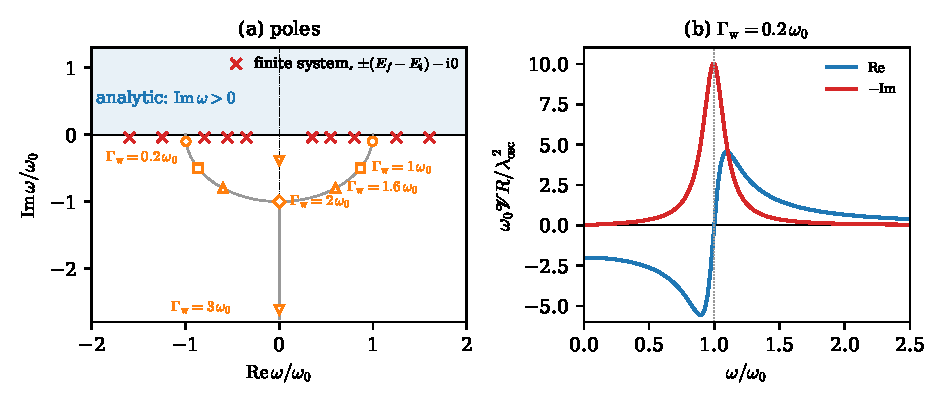
\includegraphics[width=\linewidth]{figures/ch04/fig4_1.pdf}
  \caption{Poles of the retarded response function in the complex frequency plane $\omega$, in units of an oscillator frequency $\omega_0$. (a) The response is analytic in the upper half plane (shaded). A finite target has poles at its transition energies $\pm(E_f - E_i)$, displaced by an infinitesimal $-\ii0$ below the real axis (crosses, at illustrative transition energies). A harmonic oscillator with energy damping rate $\varGamma_{\mathrm{w}}$ has poles at $-\ii\varGamma_{\mathrm{w}}/2 \pm (\omega_0^2 - \varGamma_{\mathrm{w}}^2/4)^{1/2}$ (open symbols, for the values of $\varGamma_{\mathrm{w}}$ marked). They lie on the circle $|\omega| = \omega_0$ below critical damping, $\varGamma_{\mathrm{w}} = 2\omega_0$, and on the negative imaginary axis above it; for $\varGamma_{\mathrm{w}} = 3\omega_0$ the upper of the two is at $-0.38\,\ii\omega_0$. (b) Real part and minus the imaginary part of $\Vol R$ for the damped oscillator with $\varGamma_{\mathrm{w}} = 0.2\,\omega_0$ and coupling $\lambda_{\mathrm{osc}}(d + d^\dagger)$, on the real axis. The absorptive part peaks at $2\lambda_{\mathrm{osc}}^2/\varGamma_{\mathrm{w}}$ at $\omega = \omega_0$; the real part is negative below the resonance and positive above it, and tends to $-2\lambda_{\mathrm{osc}}^2/\omega_0$ at $\omega = 0$.}
  \label{fig:4-poles}
\end{figure}

How fast $R_{ab}$ falls at large $|z|$ follows from the Lehmann form too. Expanding $1/[z \mp (E_f - E_i)] = 1/z \pm (E_f - E_i)/z^2 + \dots$ in \cref{eq:4.1-lehmann}, the coefficient of $1/z$ is the equal-time commutator, and in the coefficient of $1/z^2$ the resonant and antiresonant terms combine into a double commutator:
\begin{equation}
  R_{ab}(\vect{q},z) = \frac{\langle[O_a^\dagger, O_b]\rangle}{\Vol z} + \frac{\langle[O_a^\dagger, [H, O_b]]\rangle}{\Vol z^2} + O(z^{-3}) .
  \label{eq:4.1-tail}
\end{equation}
The coefficient of $1/z^2$ is checked by writing out $\langle i|O_a^\dagger HO_b - O_a^\dagger O_bH - HO_bO_a^\dagger + O_bHO_a^\dagger|i\rangle$ in eigenstates, which gives $\sum_f(E_f - E_i)\bigl[\langle i|O_a^\dagger|f\rangle\langle f|O_b|i\rangle + \langle i|O_b|f\rangle\langle f|O_a^\dagger|i\rangle\bigr]$. Density operators at different wavevectors commute, since both are functions of the electron positions alone, and the density response therefore falls as $1/z^2$. When the potential acting on the electrons is local, only the kinetic energy contributes to the coefficient, and the result, the f-sum rule of \cref{sec:4.3}, depends only on the electron density. For the oscillator, $[O, [H, O]] = 2\lambda_{\mathrm{osc}}^2\omega_0$, the coefficient found in \cref{we:4-oscillator}. Analyticity in the upper half plane together with this decay leads to the Kramers--Kronig relations, which reconstruct the real part of $R_{ab}$ on the real axis from its imaginary part (\cref{sec:4.3}).

\begin{workedexample}{The two-level system}\label{we:4-twolevel}
Take the two-level system of \cref{sec:2.5}: states $|0\rangle$ and $|1\rangle$ with splitting $\Delta_{\mathrm{tl}}$, Gibbs weights $p_0$ and $p_1$, and a Hermitian operator $O_a = O_b = O$ with only the off-diagonal element $O_{10} = \langle 1|O|0\rangle$. The Lehmann form \cref{eq:4.1-lehmann} has four entries. In the resonant term, $i = 0$ contributes $p_0|O_{10}|^2/(\omega - \Delta_{\mathrm{tl}})$ and $i = 1$ contributes $p_1|O_{10}|^2/(\omega + \Delta_{\mathrm{tl}})$. In the antiresonant term the same weights appear with the poles exchanged and a minus sign. Altogether,
\begin{equation}
  \Vol R(\omega) = (p_0 - p_1)\,|O_{10}|^2\left[\frac{1}{\omega - \Delta_{\mathrm{tl}} + \ii0^+} - \frac{1}{\omega + \Delta_{\mathrm{tl}} + \ii0^+}\right]
  = \frac{2\Delta_{\mathrm{tl}}\,|O_{10}|^2\tanh(\beta\Delta_{\mathrm{tl}}/2)}{(\omega + \ii0^+)^2 - \Delta_{\mathrm{tl}}^2} ,
  \label{eq:4.1-twolevel}
\end{equation}
with $p_0 - p_1 = \tanh(\beta\Delta_{\mathrm{tl}}/2)$ from \cref{eq:2.5-gibbs}. It has the form of the oscillator, \cref{eq:4.1-osc}, with $\omega_0 \to \Delta_{\mathrm{tl}}$ and $\lambda_{\mathrm{osc}}^2 \to (p_0 - p_1)|O_{10}|^2$, but now the temperature matters. At $T = \Delta_{\mathrm{tl}}/2$ the weights are 0.881 and 0.119 (\cref{fig:2-twolevel}), the response is reduced by the factor 0.762, and $\Vol R(0) = -1.523\,|O_{10}|^2/\Delta_{\mathrm{tl}}$. At $T \gg \Delta_{\mathrm{tl}}$, $\tanh(\beta\Delta_{\mathrm{tl}}/2) \to \Delta_{\mathrm{tl}}/2T$ and $\Vol R(0) \to -|O_{10}|^2/T$. For a spin $\tfrac12$ in a magnetic field, with $\Delta_{\mathrm{tl}}$ the Zeeman splitting and $O$ a transverse component of its magnetic moment, this is the Curie law of a paramagnet: the static susceptibility falls as $1/T$.

The temperature dependence comes from the weight $p_0 - p_1$. The field drives the upward transition from $|0\rangle$ and stimulated emission from $|1\rangle$ with the same matrix element, so the excited population cancels part of the absorption, and the absorbed power \cref{eq:4.1-power} is proportional to $p_0 - p_1$. Since $p_1 < p_0$ at every temperature (\cref{sec:2.5}), a two-level system in equilibrium always absorbs, and becomes transparent only as $T \to \infty$. The oscillator escapes this saturation because its matrix elements grow up the ladder: the extra absorption from level $n$, weighted by $n + 1$, exactly compensates the emission, weighted by $n$, which is why $n_{\mathrm{B}}(\omega_0)$ dropped out of \cref{eq:4.1-osc}. The tail coefficient of \cref{eq:4.1-tail} is $\langle[O, [H, O]]\rangle = 2\Delta_{\mathrm{tl}}(p_0 - p_1)|O_{10}|^2$, temperature dependent here and constant for the oscillator.

The two examples also mark where linear response stops. For the oscillator, the commutator $[O(t), O(t')]$ is a number, every nested commutator of higher order vanishes, and with it every higher-order term of the Dyson series, so \cref{eq:4.1-osc} holds at any field strength. The two-level system saturates. On resonance the field moves population between $|0\rangle$ and $|1\rangle$, and \cref{eq:4.1-twolevel} holds only while that transfer is small: the drive $|O_{10}\phi_0|$ must be small compared with the width of the transition, the weak-drive condition of \cref{app:D.3}. A stronger field makes the populations oscillate at the Rabi frequency, a response that is not linear in the field.
\end{workedexample}
